% !TEX root = ../Dokumentation.tex
\section{Technologierecherche}
\subsection{Funktionsweise der Hardware}
Für die geplante Arbeit wird ein Raspberry Pi xxx verwendet, das Raspberry Pi ist ein Einplatinencomputer und eignet sich mit seinen Funktionen und Komponenten besonders gut für diese Arbeit. Über die elektrischen Anschlusspunkte, auch GPIOs genannt, werden die Messsignale des Temperatursensors abgefragt. Mittels dem Raspberry Pi werden die gelieferten Daten der jeweiligen Sensoren von einem analogen zu einem digitalen Signal umgewandelt.
Diese Signale können so in Temperaturwerte umgerechnet und für eine kontinuierliche Anzeige bereitgestellt werden.

\begin{figure}[H]%Position festigen
\centering
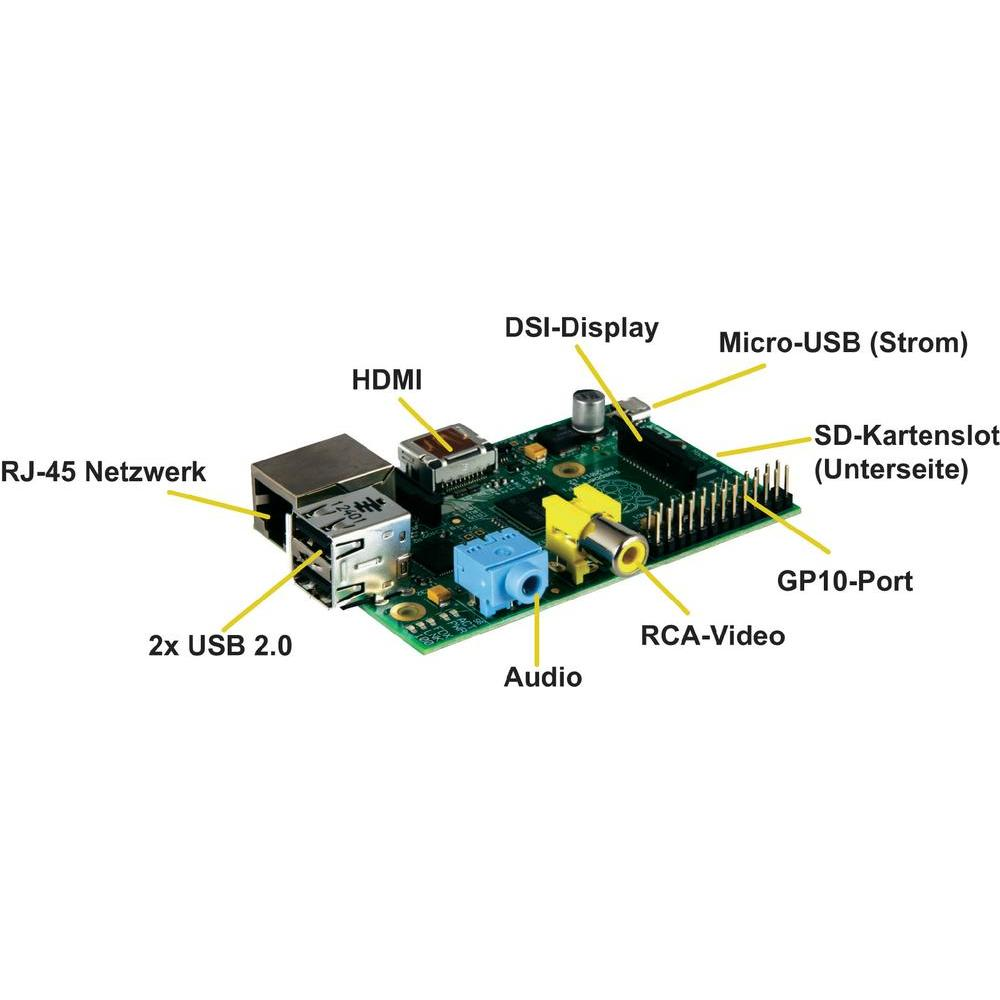
\includegraphics[width=1\textwidth]{Images/RaspberryPi.jpg}
\caption{Pi (Quelle www.Conrad.ch)}
\label{fig:raspi}
\end{figure}
\subsubsection{Raspberry}

\subsubsection{GPIO}
GPIO ist ein elektrischer Anschlusspunkt, welcher vom RaspberryPi zur Verfügung gestellt wird.

\subsection{Software Entwurfsmuster}